\documentclass[a4paper,12pt]{article}
\usepackage[utf8]{inputenc}
\usepackage[croatian]{babel}
\usepackage{verbatim}
\usepackage{listings}
\usepackage{amssymb}
\usepackage{amsmath}
\usepackage{graphicx}
\usepackage{gensymb}
\usepackage{float}

\author{Nikola~Bunjevac (0036485677)}
\title{Dokumentacija iz predmeta Interaktivna računalna grafika\\{\normalsize Inačica B}}

\begin{document}
\maketitle

\section{Prva laboratorijska vježba}

Prva laboratorijska vježba sastoji se od tri dijela---implementacije vlastite
matematičke biblioteke, pisanje prvog programa u OpenGL-u kako bismo upoznali
osnovne pojmove same specifikacije te potporne biblioteke (u ovom slučaju freeglut\footnote{http://freeglut.sourceforge.net/}) te implementacija Bresenhamovog algoritma za crtanje pravaca na rasterskim jedinicama.

U prvom dijelu prve laboratorijske vježbe trebalo je napisati vlastitu biblioteku za
rad s matematičkim objektima od presudne važnosti u računalnoj grafici, a to su vektori i matrice. Vlastita biblioteka, kao i sve ostalo, je implementirana u programskom jeziku C++. Objektno-orijentirani jezici vrlo su pogodni za rad
s računalnom grafikom jer omogućavaju elegantno definiranje i manipuliranje
potrebnim pojmovima.

Primjerice, vektori i matrice su predstavljeni posebnim
razredima, i to hijerarhijski, kako bi se postigla što veća neovisnost i
modularnost. Tako je vršni razred koji treba naslijediti svaki vektor {\verb|IVector|}, a svaka matrica {\verb|IMatrix|}. Zatim je potrebno implementirati
razrede {\verb|AbstractVector|} i {\verb|AbstractMatrix|} koji koriste
polimorfne pozive kako bi implementirali većinu funkcionalnosti, iako još
``ne znaju'' gdje će, i kako, biti smješteni u memoriji. To je upravo prednost
takve organizacije razreda. Naposlijetku, konkretni razredi {\verb|Vector|} i
{\verb|Matrix|} određuju kako će se pohranjivati elementi vektora ili matrice.

Korisno je naglasiti da, iako je ovakav dizajn vrlo elegantan i modularan, nije baš najprikladniji za programske jezike bez automatskog upravljanja memorijom (nasuprot, primjerice, Jave) pa je radi olakšanja korišten parametrizirani razred standardne biblioteke {\verb|shared_ptr<>|}.
To dosta nepovoljno utječe na performansu, što je rezultat takve organizacije.

Sada su dodane samo funkcionalnosti poput zbrajanja, oduzimanja i množenja vektora i matrica, skaliranja vektora, računanje kosinusa kuta između dvaju vektora, računanje inverza matrice, itd.
U kasnijim vježbama ćemo biblioteku proširiti razredom {\verb|IRG|} sa
statičkim metodama za stvaranje pojedinih korisnih matrica.

U drugom dijelu laboratorijske vježbe trebalo je napisati aplikaciju koja
za iscrtavanje koristi OpenGL te korisniku omogućava proizvoljno zadavanje
i crtanje trokuta unutar prozora. Korisnik klikom zadaje vrhove trokuta i
može proizvoljno mijenjati boju svakog od njih na jednu od prethodno zadanih.

OpenGL se može shvatiti kao stroj stanja. Vrhove trokuta i pripadnu boju potrebno je pamtiti u nekoj vanjskoj strukturi, a pozivi OpenGL-u se koriste tek
u trenutku iscrtavanja na ekran. Svako crtanje je strukturirano na sljedeći
način:

\begin{lstlisting}[language=C]
  glBegin(GL_*);
  // pozivi za slanje vrhova
  glEnd();
\end{lstlisting}
U ovom slučaju, argument naredbe {\verb|glBegin|} bio je {\verb|GL_TRIANGLES|}, zato što crtamo upravo trokute. Između naredbi početka i kraja, pozivima
{\verb|glVertex2f|} šaljemo 2D koordinate svakog pojedinog vrha trokuta. Kod crtanja trokuta na ovaj način, broj vrhova uvijek mora biti višekratnik broja 3, odnosno uvijek šaljemo $3n$ vrhova, gdje je
$n \in \mathbb{N}$.
Kako je OpenGL stroj stanja, boja koju postavimo u jednom trenutku će se koristiti skroz dok ne postavimo neku drugu boju. Postavljanje boje obavljamo pozivom
{\verb|glColor3f|}, koji kao argumente prima 3 broja tipa {\verb|GLfloat|}, redom crvena, zelena i plava komponenta (RGB).

U trećem dijelu vježbe bilo je potrebno implementirati Bresenhamov algoritam
za crtanje pravaca te Cohen-Sutherlandov algoritam za odsijecanje. Svaki pravac u ravnini je zadan dvjema točkama $T_1(x_1, y_1)$ i $T_2(x_2, y_2)$ i možemo ga opisati jednadžbom:
\[
y - y_1 = \frac{y_2 - y_1}{x_2 - x_1}(x - x_1)
\]
Crtanje u ovom obliku je itekako moguće, ali pod cijenu loših performansi.
Ideja Bresenhamovog algoritma je optimizirati postupak crtanja pravca, i to
na više načina. Osnovna ideja je da se ne računa cijeli izraz u svakom koraku, već da se prati gomilanje pogreške (udaljenosti od sljedećeg piksela) te se nakon određene vrijednosti pomaknemo za jedan piksel u odgovarajućem smjeru i
resetiramo pogrešku. Tako će pogreška uvijek biti mali broj.
Nagib pravca možemo izračunati samo jednom i koristiti ga u svakom koraku.

Druga ideja je raditi s cijelim brojevima umjesto s brojevima s pomičnim zarezom. Time se postiže veća brzina, te ne moramo paziti na numeričku stabilnost.

Cohen-Sutherlandov algoritam služi za odsijecanje nevidljivih dijelova
objekata koje crtamo. Primjerice, kod pravaca crtamo samo  segment koji je
vidljiv na ekranu. Algoritam se temelji na ideji da cijelu površinu podijeli
na dijelove i svakome pridružimo binarni kod koji opisuje prolazi li objekt
tim dijelom. Nakon toga je, ovisno o binarnom kodu, potrebno korigirati
granice objekta tako da se cijeli objekt nalazi u vidljivom području (kod 0000).

\section{Druga laboratorijska vježba}

Druga laboratorijska vježba sastojala se od dva dijela. U prvom dijelu trebalo je napisati OpenGL
program za crtanje i popunjavanje poligona. Taj zadatak je jedan od najčešćih u računalnoj grafici
te je često sklopovski podržan od grafičke kartice. Ipak, korisno je znati kako taj postupak obaviti
``ručno''.

Poligon je geometrijski lik koji se sastoji od $n$ vrhova i $n$ linijskih segmenata (bridova) koji ih povezuju. Najjednostavniji poligon je trokut, koji se vrlo često koristi za definiranje ostalih poligona.
Trokut je relativno jednostavan, a svaki poligon s više od 3 vrha se može prikazati pomoću više
trokuta. Primjerice, pravokutnik možemo podijeliti na dva trokuta. 3D modele možemo predstaviti
pomoću mreže poligona, odnosno trokuta. Stoga je vrlo važno moći brzo i efikasno obrađivati te
iscrtavati poligone, ili jednostavnije, trokute.

Poligoni mogu biti konveksni ili konkavni. Odaberimo dvije proizvoljne točke $T_1$ i $T_2$ koje se
nalaze unutar poligona. Poligon je konveksan ukoliko linija koja povezuje točke $T_1$ i $T_2$ ne siječe
niti jednu stranicu poligona. U protivnom, poligon je konkavan. Stranice poligona možemo predstaviti već navedenom jednadžbom pravca.
Još jedan zgodan način za zapamtiti pojam konkavnosti jest da u udubinu konkavnog poligona možemo uliti kavu.

Drugo važno svojstvo poligona je smjer u kojemu su zadani njegovi vrhovi. To su dva moguća smjera---u smjeru kazaljke na satu
(engl. {\sl clockwise}) i suprotno od smjera kazaljke na satu (engl. {\sl counter-clockwise}).
Smjer zadavanja vrhova između ostalog određuje smjer normale ravnine u kojoj leži poligon te s koje
strane bridova se nalaze ostalih vrhovi.

Definirat ćemo pojam strane na koje se točka nalazi u odnosu na pravac. Neka je pravac zadan
jednadžbom
\[
  y = ax + b
\]
gdje je $a$ nagib pravca. Uvrštavanjem točke $T(x, y)$ u jednadžbu pravca dobit ćemo broj koji
može biti pozitivan, negativan ili 0. Ukoliko je rezultat pozitivan, točka se nalazi {\sl iznad}
pravca, ako je rezultat negativan, točka se nalazi {\sl ispod} pravca, a ako je rezultat 0, točka
leži na pravcu. Drugi način za shvaćanje je da zamislimo da se nalazimo na pravcu i gledamo u
smjeru od početne do krajnje točke kojima je pravac zadan. S lijeve strane nam se nalaze sve točke
koje su iznad pravca, s desne strane sve točke koje su ispod pravca, a točno ispred i iza nas se
nalaze sve točke koje leže na pravcu.

Sada ćemo opisati kako ispuniti konveksni poligon bojom. Postupak se temelji na principu skenirajuće linije
(engl. {\sl scanline}). Potrebno je odrediti najmanji pravokutnik koji omeđuje poligon (engl. {\sl AABB, axis-aligned bounding box}). Uz pretpostavku ekranskog koordinatnog sustava, ideja je krenuti
od najmanje $y$ koordinate poligona i ići redom po svim $y$ koordinata do najveće koja je obuhvaćena poligonom.
Na svakoj $y$ koordinati potrebno je odrediti $x$ koordinate sjecišta pravca $y = b$ s bridom poligona.
Nakon što smo odredili sjecišta, potrebno je nacrtati linijski segment koji spaja dva sjecišta.
Kako smo pretpostavili da se radi o konveksnim poligonima, algoritam možemo i malo ubrzati na način
da sortiramo bridove od vrha prema dnu te u svakom koraku razmatramo samo dva brida koji se nalaze
na trenutnoj $y$ koordinati. Taj postupak je korišten u vlastitoj implementaciji. Prikaz
poligona popunjenog navedenim algoritmom prikazan je na slici \ref{fig:polygon}.

\begin{figure}[H]
  \centering
  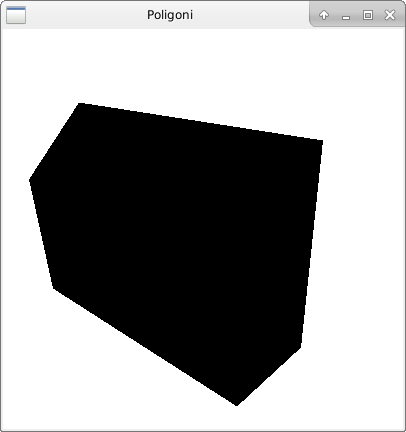
\includegraphics[width=0.5\textwidth]{img/polygon.png}
  \caption{Prikaz popunjavanja poligona}
  \label{fig:polygon}
\end{figure}

Program je trebao korisniku omogućiti nekoliko opcija. Sastoji se od dva stanja---zadavanja poligona te provjere odnosa točke i poligona. Pritiskom na tipku {\tt k} moguće je
birati smije li se zadati samo konveksan poligon ili i konkavan. Ukoliko je zastavica postavljena,
novih vrh koji bi poligon učinio konveksnim mora se odbiti postaviti. Tipka {\tt p} omogućava
popunjavanje poligona. Tipkom {\tt n} ciklički se prelazi u iduće stanje. U stanju zadavanja
se klikom miša odabiru vrhovi poligona. U stanju provjere odnosa točke i poligona se klikom miša
odabiru koordinate točke za koju se želi izvršiti provjera. Prelaskom iz stanja provjere u stanje
zadavanja poligona brišu se svi do tada zadani vrhovi. Ova vježba je
implementirana koristeći OpenGL 3.3 te biblioteku GLFW\footnote{http://www.glfw.org/}. 

Drugi dio vježbe sastojao se od učitavanja trodimenzionalnog tijela iz {\tt .obj} datoteke te
provjere odnosa od korisnika zadane točke i objekta. {\tt .obj} datoteka sadrži niz definicija
koje opisuju kako objekt izgleda u prostoru. Vrhove je moguće definirati navođenjem znaka {\tt v}
nakon kojega se nalaze tri koordinate $(x, y, z)$. Trokute, odnosno ravnine je moguće zadati
navođenjem znaka {\tt f} iza kojega se nalaze tri indeksa (počevši od 1) koji predstavljaju tri vrha.

Nakon učitavanja objekta iz datoteke, potrebno je izračunati određene parametre. Za svaki trokut
možemo odrediti ravninu u kojoj se nalazi i predstaviti ju jednadžbom
\[
ax + by + cz + d = 0
\]
gdje je $[a\ b\ c]^T$ normala ravnine izračunata pomoću vektorskog produkta bridova. Definirano je
da normala uvijek pokazuje ``prema van'' i vrhovi trokuta su zadani na način koji to osigurava.
Normalu računamo kao $\mathbf{n} = v_{i}v_{i+1} \times v_{i}v_{i+2}$, gdje je $v_iv_j$ vektor koji
ide od vrha $v_i$ prema vrhu $v_j$.

Nakon uspješnog učitavanja modela, korisnik u konzoli može upisivati 3D
koordinate i provjeravati nalazi li se točka unutar, izvan ili na obodu objekta,
naredbom {\tt normaliziraj} može normalizirati objekt tako da se nalazi
unutar kocke dimenzija $[-1, 1]$ oko ishodišta, te će mu se u konzoli ispisati
{\tt .obj} zapis normiranog objekta.
Naredbom {\tt quit} završava rad programa.

\section{Treća laboratorijska vježba}

Teme treće laboratorijske vježbe bile su projekcije, uklanjanje skrivenih poligona te B{\'e}zierova krivulja. Projekcije
su ključan pojam računalne grafike jer one čine prikaz trodimenzionalnih prostora i objekata
mogućim. Postoje dvije važnije vrste projekcija, a to su:
\begin{enumerate}
  \item perspektivna i
  \item paralelna.
\end{enumerate}

Paralelna projekcija, kao što joj i ime govori, čuva paralelnost pravaca nakon projekcije. Ipak,
bavit ćemo se perspektivnom projekcijom koja je bliža ljudskom vidu i poimanju prostora oko nas.
Karakterizira je to što su dalji objekti manji, a bliži objekti veći.
Ideja je da odredimo volumen pogleda, krnju piramidu (engl. {\sl frustum}), koja predstavlja
prostor ispred promatrača koji on može vidjeti. Sve što se nalazi izvan volumena pogleda, neće biti
prikazano na ekranu. Volument pogleda određen je s nekoliko parametara, a to su primjerice
$f_{near}$ i $f_{far}$ koji predstavljaju udaljenost bliže i dalje plohe od promatrača, zatim
parametri $t$, $b$, $r$, $l$ koji efektivno određuju širinu i visinu bliže plohe. Drugi način za
određivanje dimenzija bliže plohe je korištenje kuta gledanja (engl. {\sl field of view}).
Taj način koristi naredba {\verb|gluPerspective|}.

Osim korištenja funkcija koje nudi OpenGL i pomoćne biblioteke, trebalo je implementirati i
``ručnu'' perspektivnu projekciju koristeći pripadnu matricu:
\[
\begin{bmatrix}
  \frac{2n}{r - l} & 0 & 0 & 0\\
  0 & \frac{2n}{t - b} &  0 & 0\\
  \frac{r + l}{r - l} & \frac{t + b}{t - b} & -\frac{f + n}{f - n} & -1\\
  0 & 0 & -\frac{2fn}{f - n} & 0
\end{bmatrix}
\]

Množenjem točke matricom dobivamo projiciranu točku. Što se zapravo događa
prilikom ove operacije? Zamislimo krnju piramidu pogleda. Uži kraj neka je
bliži promatraču (nama). Prilikom perspektivne projekcije, volumen pogleda i
sve što se nalazi unutar njega se transformira u kocku stranice duljine 1.
Stoga će ono što je bliže nama biti veće, a ono što je dalje će biti manje.
Dalji kraj krnje piramide je širi i on će se suziti, a bliži kraj je uži i
on će se proširiti čime dobivamo prikaz analogan stvarnom svijetu.

Program omogućava učitavanje trodimenzionalnih objekata kao u prethodnoj
vježbi navođenjem puta do {\verb|.obj|} datoteke. Također je implementirana
animacija objekta u smislu da se objekt rotira oko svoje osi. Tipkama
{\tt r} i {\tt l} se može ručno rotirati objekt oko svoje osi. Tipkom
{\tt ESC} se kut gledanja resetira na početnu vrijednost.

U drugom dijelu vježbe bilo je potrebno implementirati nekoliko algoritama
za skrivanje nevidljivih površina. Razlog implementacije takvih algoritama
je što nema potrebe za iscrtavanjem nečega što korisnik uopće ne vidi zbog
čega dobivamo bolje performanse. Velike scene mogu sadržavati tisuće ili
milijune trokuta od kojih ponekad i više od polovice ne vidimo. Vidimo
da je korist takvih postupaka velika, a algoritmi kojima se to postiže
relativno jednostavni. Algoritme možemo podijeliti u dvije skupine:
\begin{enumerate}
  \item u prostoru objekata/scene
  \item u prostoru piksela.
\end{enumerate}

Prva skupina se odvija prije projekcije, dok se druga skupina odvija nakon
projekcije.

Iz prve skupine su implementirana dva algoritma. Jedan se temelji na odnosu
očišta i jednadbžbe ravnine u kojoj poligon leži, a drugi se temelji na
odnosu vektora normale poligona i vektora koji ide od centra poligona prema
očištu.

Pogledajmo kako radi prvi algoritam. Neka je očište definirano vektorom
$\mathbf{eye} = [eye_x\ eye_y\ eye_z\ 1]^T$, a jednadžba ravnine neka je
$ax + by + cz + d = 0$. Uvrštavanjem vrijednosti vektora očišta u jednadžbu
ravnine dobivamo $s = a{eye_x} + b{eye_y} + c{eye_z} + d$. Ako je $s < 0$, onda je
poligon stražnji i nije ga potrebno iscrtavati.

U drugom algoritmu potrebno je izračunati centar poligona što možemo učiniti
na sljedeći način: $\mathbf{c} = \frac{v_i+v_{i+1}+v_{i+2}}{3}$, jer se radi
o trokutu. Definirajmo vektor $\mathbf{e} = \mathbf{eye} - \mathbf{c}$ te
neka je $\mathbf{n}$ normala poligona. Pogledajmo sada kut između vektora
$\mathbf{n}$ i $\mathbf{e}$ kojega možemo izračunati pomoću skalarnog produkta. Ako je kut iz intervala $(-90\degree, +90\degree)$, poligon je prednji i
ne smijemo ga zanemariti, dok je u ostalim slučajevima stražnji i nije ga potrebno
iscrtavati.

Treći algoritam radi u prostoru piksela i temelji se na smjeru iscrtavanja
vrhova poligona (u ovom slučaju trokuta, ali rezultat se može primijeniti i
na ostale konveksne poligone). Ideja je da nakon projekcije, prije crtanja
provjerimo u kojem smjeru je potrebno iscrtavati vrhove poligona. Ukoliko je
smjer istovjetan smjeru kazaljke na satu, poligon je stražnji i možemo ga
zanemariti. Primijetimo kako ovaj postupak ne zahtijeva nikakve dodatne
informacije (kod prošlih smo morali znati očište). Iz tog razloga ga koristi
OpenGL ukoliko korisnik traži opciju skrivanja stražnjih poligona (engl.
{\sl backface culling}).

Korisno je napomenuti kako sva tri algoritma daju identične rezultate, a
treći je dao najsporije iz razloga što su se svi objekti prvo projicirali pa
se tek onda vršila potrebna provjera, što kod ostala dva algoritma nije bio
slučaj. Rezultat je prikazan na slici \ref{fig:teapot}.

U posljednjem dijelu laboratorijske implementiran je prikaz B{\'e}zierove
krivulje. Korisnik može klikom miša zadavati kontrolne točke. Desnim klikom
može pomicati pojedinu kontrolnu točku. Na ekranu se iscrtava kontrolni poligon,
aproksimacijska krivulja te interpolacijska krivulja koja prolazi svim točkama
kontrolnog poligona. Rezultat je prikazan na slici \ref{fig:bezier}.
\begin{figure}[H]
  \centering
  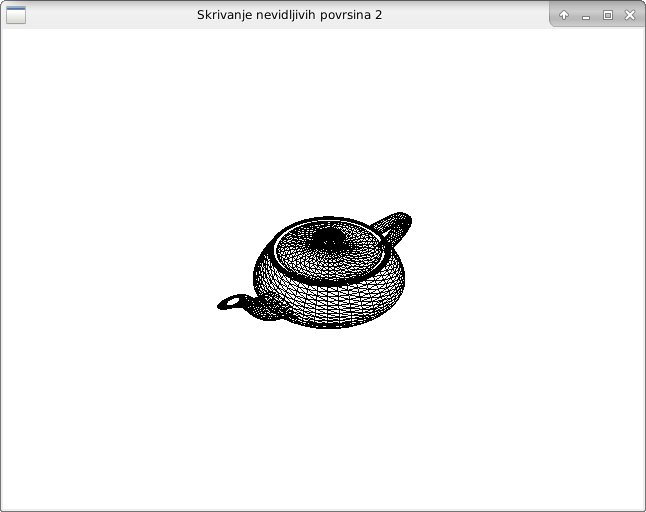
\includegraphics[width=0.8\textwidth]{img/surface_hiding.png}
  \caption{Skrivanje nevidljivih poligona}
  \label{fig:teapot}
\end{figure}

\begin{figure}[H]
  \centering
  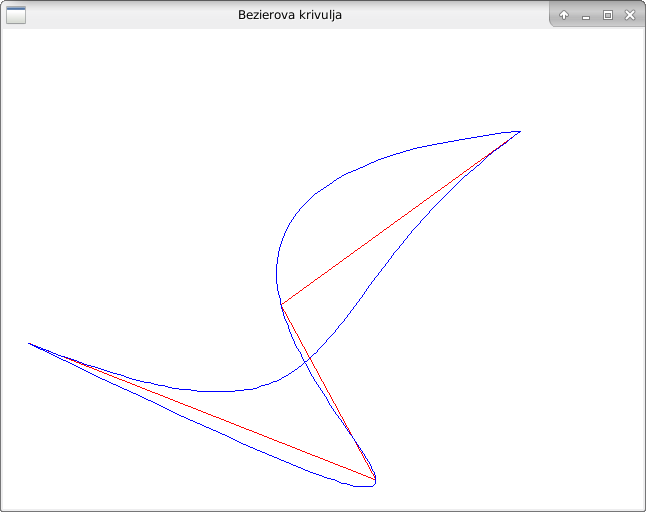
\includegraphics[width=0.8\textwidth]{img/bezier.png}
  \caption{Prikaz B{\'e}zierove krivulje}
  \label{fig:bezier}
\end{figure}

\section{Četvrta laboratorijska vježba}

U posljednjoj laboratorijskoj vježbi odlučio sam se za izradu {\sl raytracera}, odnosno implementaciju
algoritma praćenja zrake. Algoritam je u osnovi vrlo jednostavan, a vizualno daje iznimno dobre rezultate.
Model koji primjenjuje se nalazi između empirijskog i fizikalnog/analitičkog. Naime, temelji se
na pretpostavci da se svjetlost širi pravocrtno, što naravno, nije uvijek istina. Glavna prednost
je što su sjene automatski ``uključene'' u model, kao i refleksije, odnosno zrcalne površine.
Algoritam možemo opisati sljedećim pseudokodom:
\begin{verbatim}
  za svaki piksel (x, y) ekrana:
    točka T = pretvori (x, y) u 3D koordinate proj. ravnine
    ispucaj zraku koja ide od promatrača i prolazi kroz točku T

    ako  je došlo do sudara zrake i objekta:
      izračunaj boju
      boja += rekurzivno izračunaj boju reflektirane zrake
    kraj ako 
\end{verbatim}

Jednostavnija varijanta je algoritam bacanja zraka koji je lokalni model osvjetljenja iz razloga
što se boja računa samo u prvoj točki sudara zrake i objekta. Algoritam praćenja zrake uvodi
proširenje da prilikom sudara nastavlja praćenjem reflektirane ili lomljene zrake.

Program kao argument prihvaća put do datoteke koja sadrži opis scene. Datoteka mora sadržavati
gledište, udaljenost projekcijske ravnine od gledišta, kuteve po $x$- i $y$-osi koji određuju
širinu i visinu projekcijske ravnine, vektora smjera pogleda, {\sl view-up} vektora te intenzitet
globalnog ambijentnog osvjetljenja. Nakon toga je potrebno definirati objekte u prostoru.
Podržane su dvije vrste objekata---krpice i kugle. Svaki objekt je opisan s nekoliko parametara,
točkom koja predstavlja centar objekta, kuglu još opisuje radijus, a krpice dva nekolinearna vektora
te širina i visina krpice u jedinicama zadanih vektora.
Također je potrebno još opisati i kako objekt međudjeluje sa svjetlosti. Kako se koristi empirijski
Phongov model osvjetljenja, potrebno je definirati tri komponente:
\begin{enumerate}
  \item ambijentnu
  \item difuznu i
  \item zrcalnu.
\end{enumerate}

Komponente su definirane kao faktori koji se množe s intenzitetom točkastog svjetla u prostoru.
Kod krpica je potrebno definirati faktore osvjetljenja i za prednju i za stražnju stranu, dok
kod kugle pretpostavljamo da se promatrač neće nalaziti unutar kugle pa definiramo samo prednju
stranu. Točka $\mathbf{p}$ se nalazi na prednjoj strani ukoliko je skalarni produkt
$\mathbf{p} \cdot \mathbf{n} > 0$, gdje je $\mathbf{n}$ normala u točki površine objekta.

Zanimljivo je napomenuti da algoritam daje vrlo realistične rezultate, gotovo kao da se nalazimo
na mjestu promatrača. Najveći nedostatak je računska zahtjevnost postupka, ali uz dobro
strukturiranje i imutabilnost moguće je postići visoki stupanj paralelizacije/višedretvenosti,
a samim time o bolju performansu. U praksi postoje brojne implementacije, a jedan od zanimljivijih
i poučnijih je {\tt pbrt}\footnote{http://www.pbrt.org/} koji se temelji na vrlo realističnom
modelu temeljenom na fizici (engl. {\sl Physically based rendering}).

\begin{figure}[H]
  \centering
  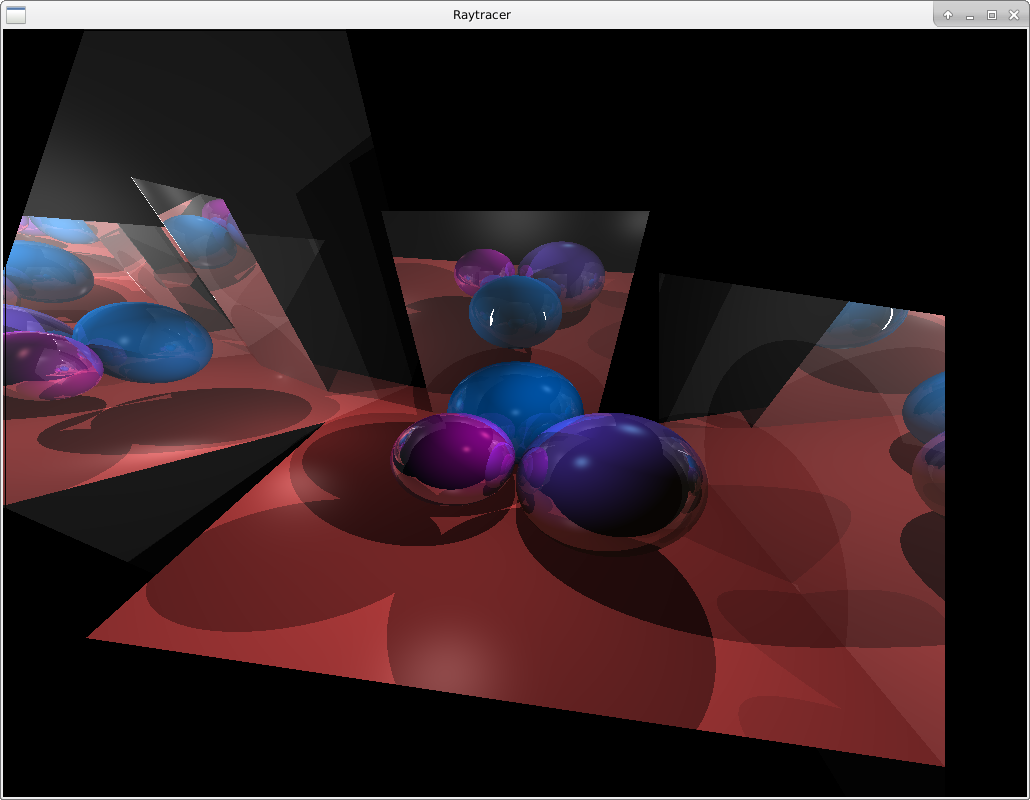
\includegraphics[width=0.8\textwidth]{img/simple_scene.png}
  \caption{Rezultat rada algoritma praćenja zrake}
  \label{fig:raytracer}
\end{figure}

U drugom dijeli vježbe implementirani su programi koji računaju fraktale. Fraktali su vrlo
zanimljivi matematički pojmovi koje karakterizira samoponavljanje i vrlo detaljna struktura.

Prvi obrađeni fraktal je Mandelbrotov fraktal definiran pomoću kompleksnih brojeva.
Definirajmo funkciju $f$ na sljedeći način:
\[
f(z) = z^2 + c;\quad z, c \in \mathbb{C}
\]
gdje je $c$ kompleksni broj za koji želimo provjeriti pripadnost Mandelbrotovom skupu.
Mandelbrotov skup je definiran kao skup svih kompleksnih brojeva za koje funkcija $f$ ne
divergira. Što bi značilo da ne divergira? To znači da iterativno uvrštavamo broj $z$ u funkciju
$f$, uz početnu vrijednost 0. Granicu divergencije definiramo kao krug radijusa 2. Ukoliko
nakon zadanog broja iteracija vrijednost ne prijeđe granicu, broj $c$ ćemo označiti kao da pripada
skupu. Rezultat je prikazan na slici \ref{fig:mandelbrot}. Primijetimo sada da svaki broj divergira
u određenom broju koraka koji ne mora nužno uvijek biti isti. Možemo tom broju koraka pridružiti boju,
a rezultat će biti interesantan prikaz koji se naziva Mandelbrotov fraktal.
Program omogućava izmijenjivanje crno-bijelog prikaza te prikaza u boji
pritiscima na tipke {\tt c} ili {\tt b}, a desnim klikom miša dobit će se
uvećani prikaz područja oko pokazivača miša. Također je moguće prikazati
Mandelbrotov fraktal koji u funkciji $f$ koristi $z^3$ umjesto $z^2$ pritiskom
na tipku {\tt 2}. Kako bi se olakšalo zumiranje, implementirano je spremanje
vrijednosti na stog koje se može koristiti tipkom {\tt x}. Tipkom {\tt ESC}
parametri prikaza se vraćaju na početne.

\begin{figure}[H]
  \centering
  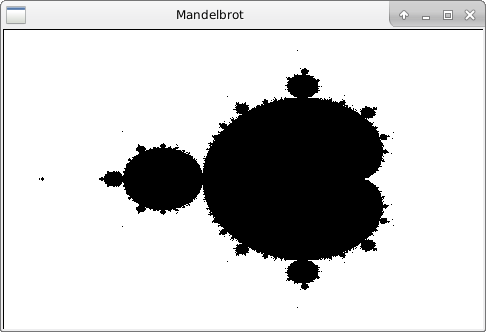
\includegraphics[width=0.8\textwidth]{img/mandelbrot.png}
  \caption{Prikaz Mandelbrotovog skupa}
  \label{fig:mandelbrot}
\end{figure}

Kao druga vrsta fraktala implementiran je IFS fraktal (engl. {\sl Iterated Function System}).
Njegova ideja je definirati fraktal kao skup transformacija oblika
\[
\begin{bmatrix}
  x'\\
  y'
\end{bmatrix}
=
\begin{bmatrix}
  a & b\\
  c & d
\end{bmatrix}
\begin{bmatrix}
  x\\
  y
\end{bmatrix}
+
\begin{bmatrix}
  e\\
  f
\end{bmatrix}
\]
pri čemu je svakoj transformaciji pridružena određena vjerojatnost. Naravno,
zbroj svih vjerojatnosti mora biti jednak 1. Nakon što je definiran sustav
transformacija u datoteci, program iterativno računa točke fraktala u
unaprijed zadanom broju iteracija i to tako da svaki put transformira
početnu točku nekom transformacijom, zatim novu točku opet transformira nekom
transformacijom itd. Koja će transformacija biti odabrana bira se slučajno,
ali u ovisnosti o pridruženoj vjerojatnosti---transformacije s većom
vjerojatnosti biti će češće odabrane od onih s manjom pridruženom vjerojatnosti. Na slici \ref{fig:sierpinski} je prikazan interesantan fraktal u obliku
trokuta koji se naziva trokut Sierpi{\'n}skog. Definiran je na način
da zamislimo da imamo veliki trokut čiji je donji lijevi kut na koordinati
$(0, 0)$. Zatim definiramo tri transformacije s jednakom vjerojatnosti, od
kojih svaka skalira trokut za $1/3$, te ga translatira u donji desni
ugao, u gornji ugao ili ga pak ne translatira, odnosno ostavlja ga u donjem
lijevom uglu.

\begin{figure}[H]
  \centering
  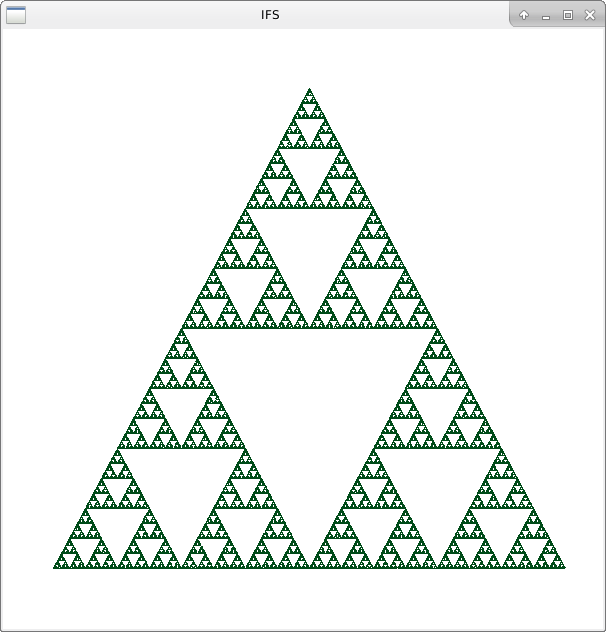
\includegraphics[width=0.8\textwidth]{img/sierpinski.png}
  \caption{Prikaz trokuta Sierpi{\'n}skog}
  \label{fig:sierpinski}
\end{figure}

\end{document}
